\clearpage\section{Results}

% {This should include your data analysis and findings}

% \begin{figure}[H]
% \label{fig:prototype1}
% \centering
% 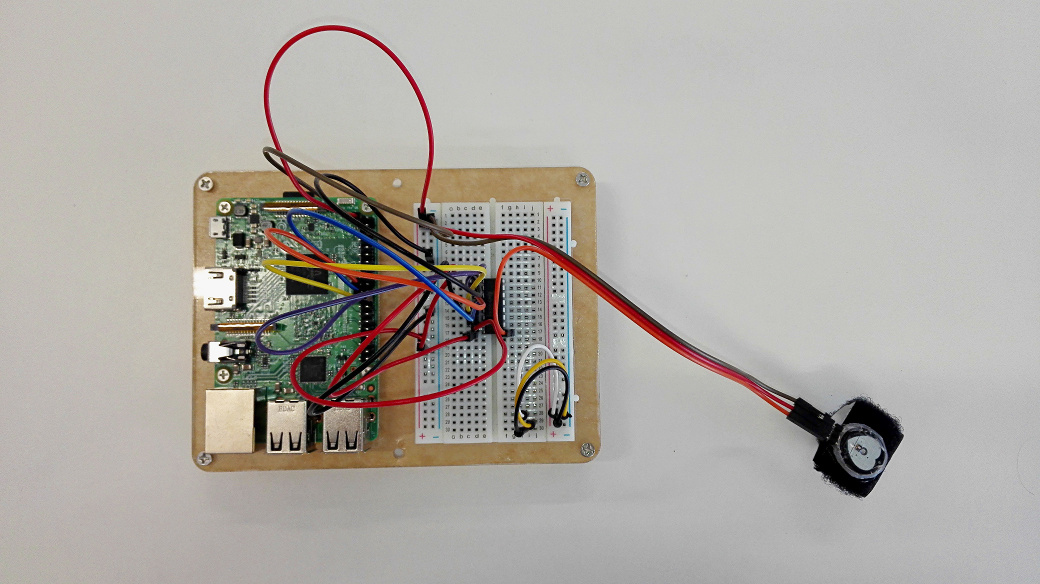
\includegraphics[width=10cm]{img/Chapter4/prototype1_edited.jpg}
% \caption[Prototype setup]{\footnotesize{Prototype setup.}}
% \end{figure}

% \begin{table}[H]
% \centering
% \caption[This is the caption]{ \footnotesize This is the other caption. Since the trial size of the experiments showed is one second, the number of \textit{Target} and \textit{Impostor} data corresponds to number of trials or seconds}
% \label{tab:data_partition}
% \footnotesize{
% \begin{tabular}{@{}llcccc@{}}
% \toprule
% \textbf{Dataset}         & \multicolumn{1}{c}{\textbf{Label}} & \textbf{Train} & \textbf{Validation} & \textbf{Develop} & \textbf{Test} \\ \midrule
% \midrule
% \multirow{3}{*}{First} & Target   & $135$ & $45$  & $30$  & $30$  \\
%                          & Impostor & $5,220$    & $1,740$ & $1,890$   & $2,880$    \\
% \cmidrule(lr){3-5} \cmidrule(l){6-6}
%                          & \#Subjects          & \multicolumn{3}{c}{$31$} & $12$ \\
% \midrule
% \multirow{3}{*}{Second}  & Target   & $144$ & $80$  & $48$  & $48$  \\
%                          & Impostor & $2,014$    & $1,119$    & $1,343$    & $1,545$ \\
% \cmidrule(lr){3-5} \cmidrule(l){6-6}
%                          & \#Subjects   & \multicolumn{3}{c}{$15$} & $5$ \\ 
% \bottomrule
% \end{tabular}
% }
% \end{table}

% \begin{algorithm}
\caption{Temperature-Distributed algorithm}\label{alg:tempdistrib}
\begin{algorithmic}[1]
\Procedure{Temp-Spread}{$GN_i, HN_j, temperatures$}\Comment{Lowest temperature priority}
\State $temperature\_list\gets short(temperatures)$
\State $max_temperature\gets max(temperature_list)$
\State $ThresHold\gets 0.5$
\State $temperature\_impact \gets 0.2$
\For{$GN_i$ in $i=1,8$}\Comment{Iterate every hardware node on the given GN}
\State $it\_temperature \gets temperature\_list(GN_i)$
\State $temp\_weight \gets \frac{max\_temperature-it\_temperature}{max\_temperature}*temperature\_impact$
\State $\omega(Master-GN_i) \gets ThresHold*temp\_weight$
\For{$HN_j$ in $j=1,n$}
\If{$available\_accel_{i,j} > busy\_accel_{i,j}$}
    \State $policy_\omega = \frac{Available HW}{Total HW}*ThresHold$
    \State $\omega(GN_i-HN_{i,j}) \gets ThresHold+policy_\omega$
\Else
    \State $\omega(GN_i - HN_{i,j}) \gets 1$
\EndIf

\EndFor
\EndFor
\State $node \gets find\_djistra\_shortest\_path(Master\_Node, aux\_node)$
\State \textbf{$return node$} $b$\Comment{The gcd is b}
\EndProcedure
\end{algorithmic}
\end{algorithm}

\subsection{Optimization of the code}

The first bottleneck found in the process of computing the histogram was the construction of the matrix $M$ itself. In the first iterations of the code we weren't considering the possibility of parallelizing, or even vectorizing the operations. When speaking of \textit{vectorizing} we refer to the use of numpy arrays and operations, which are optimized for numerical operations.

The initial implementation of the $M$ matrix calculation consisted on computing the matrix elements in a serial way, applying the hankel function to each element of the matrix. The approximate time of computing the whole matrix of dimension $N\times N \approx 700\times 700$ was around 20 seconds. Then, exploiting the fact that the matrix is symmetric, the time was reduced to around 10 seconds.

After this, an arcaic parallelisation scheme was proposed: the matrix was divided in four triangular blocks [make figure], and each block was computed in a different process. This computation was done initializing 4 different jobs with the multiprocessing library, and then joining the results. With this we achieved a time of 2.5 seconds for the whole matrix. Even though, the time was reduced by a factor of 8, it was still the bottleneck of the computation.

Finally, thanks to some training done externally, and by rethinking the way in which the matrix is constructed, the construction stopped being the bottleneck. With the help of the fact that numpy and scipy functions are optimized to work with array-like data, the construction was thought as follows:

\begin{enumerate}
    \item From the list of scatterers (array of dimension $(N,2)$ consisting on 2D vectors representing the coordinates of each scatterer) an upper diagonal matrix (without diagonal) is constructed, consisting on the value of the distance of dispersor $i$ with dispersor $j$. That is:
    \begin{equation}
        \mathcal{D}_{ij}=\begin{cases}
            |r_i-r_j|& i<j\\
            0&else
        \end{cases}
    \end{equation}
    This matrix is computed using numba's njit decorator [ANNEX?]
    \item This matrix is then multiplied by the momentum of the free particle. This basically is an upper triangular matrix that contains the argument of the hankel function.
    \item Then, the hankel function is applied once to the whole matrix, reducing the for loops needed.
    \item The transposed matrix is added to the upper triangular matrix.
    \item Finally, the diagonal is added.
\end{enumerate}

\subsection{Density of localized states}

The sign of a localized state is the exponential decay of the wavefunction $\psi\propto e^{-\frac{r}{\xi}}$ far from the source. When working with the Green's function, we don't work with exactly the wavefunction, but with the correlation function. In this case, a localized state has an exponential decay of the correlator, but the exponential decay of the correlator does not imply localization. This is because the state can lie in a spectral gap of the system, where the correlator decays exponentially [REFERENCE], and, in fact, this is shown in the appendix A of [Massignan Castin 2006]. 

In the scope of this study, we will study the density of localized states, that is, we will study the presence of localized states as a function of the energy $E$ of the matter wave. This study lets us discard the spectral gap, as the spectral gap is an energy range in which no state is allowed.

Following \cite{antezzaQuantitativeStudyTwo2010}, a localized state is expected to correspond to a very narrow ressonance inside the scattering medium. That is, a localized state corresponds to a pole of the analytically continued Green's function in the lower plane $\Gamma >0$: \textcolor{red}{Why is this? and why gamma over 2?}

\begin{equation}
    z_{res}=E_{res}-i\hbar \frac{\Gamma}{2}
    \label{eq:resonance}
\end{equation}

Using a disordered circular lattice of scatterers of radius $R=150d$ and occupation probability $p=0.1$, for a mean number of scatterers $\langle N\rangle \approx 7\cdot 10^3$, we can compute for some energies the mean width of the ressonances found. The results are shown in \cref{fig:loc_states}. By construction of the matrix $M$, we can see that the number of eigenvalues of the matrix is equal to the number of dispersors, meaning in this case that we will have for each energy $E$ around $7\cdot 10^3$ potential ressonances. Applying the Newton's method mentioned before, we can identify a scattering length $a_{eff}$ for each eigenvalue of the matrix, which is shown in \cref{fig:num_states}. It is interesting to note that for a small value of the energy, the number of states found for $a_{eff}<d$ (or $\ln(a_{eff}/d)<0$) is zero, meaning that there are no states available there. For this reason, we will particularize on the states with $a_{eff}=d$.

We can define the surface participation ratio as:

\begin{equation}
    S_p=\frac{1}{\rho \sum_{i=1}^N|D_i|^4}
\end{equation}

Where $\rho\equiv \frac{p_{occ}}{d^2}$ is the average density of scatterers, and $D_i$ is the $i$-th component of the eigenvector corresponding to the state. Looking at the wavefunction \cref{eq:wavefunction_resonance}, we can see that this quantity is inversely proportional to the Inverse Participation Ratio, which in general is defined as:

\begin{equation}
    IPR=\sum_{i=1}^N|\psi_i|^4
\end{equation}

And it is a usual metric to determine how much a state is spreaded through the system. In lattice systems, an IPR of 1 means that the state is localized in a single site, while an IPR of $N$ means that the state is spreaded through all the system.

Then, if we search for states with $S_p^{\frac{1}{2}}<\alpha d^2$, with $\alpha>0$, we will throw away states which are spreaded through the system.

\begin{figure}[ht]
    \centering
    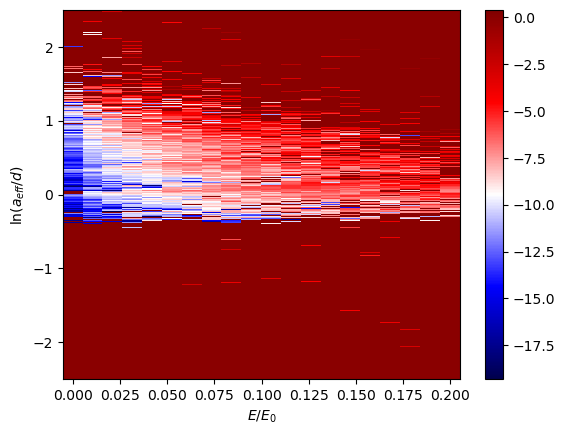
\includegraphics[width=0.7\textwidth]{img/histogram.png}
    \caption{Width $\Gamma$ of the ressonances as a function of the energy $E$ of the matter wave. The color of each bin is computed as the base 10 logarithm off the arithmetic mean of the width of the ressonances in that bin, that is, for each bin $i$ we compute $\log_{10}\left(\frac{1}{N_i}\sum_{j\in i}\Gamma_j\right)$, where $N_i$ is the number of ressonances in the bin. The width of the bins is $\delta E=0.01E_0$ and $\delta \ln a_{eff}=0.007d$. The system used is a disordered circular lattice of scatterers of radius $R=150d$ and occupation probability $p=0.1$. The result has been filtered such that the participation surface of the state is $S_p^{\frac{1}{2}}<9.5d$.}
    \label{fig:loc_states}
\end{figure}

\begin{figure}[ht]
    \centering
    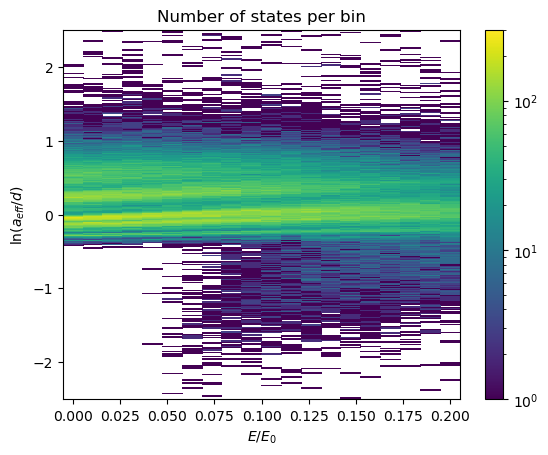
\includegraphics[width=0.7\textwidth]{img/statistics.png}
    \caption{Number of states $N_i$ found for each bin $i$. The color scale is in logarithm scale, a white value means that no state was found in that bin. The parameters used are the same as in \cref{fig:loc_states}.}
    \label{fig:num_states}
\end{figure}
\clearpage

\subsection{The wavefunction}

With \cref{eq:wavefunction_resonance}, we can explore the different kinds of wavefunction that we can find in the system. In \cref{fig:localized_state} we can see the wavefunction of a localized state with energy $E=0.005E_0$ and scattering length $a_{eff}=d$. As it can be seen in the picture the wavefunction only spans a few units of $d$ around its maximum, and decays exponentially far from the source.

\begin{figure}[ht]
    \centering
    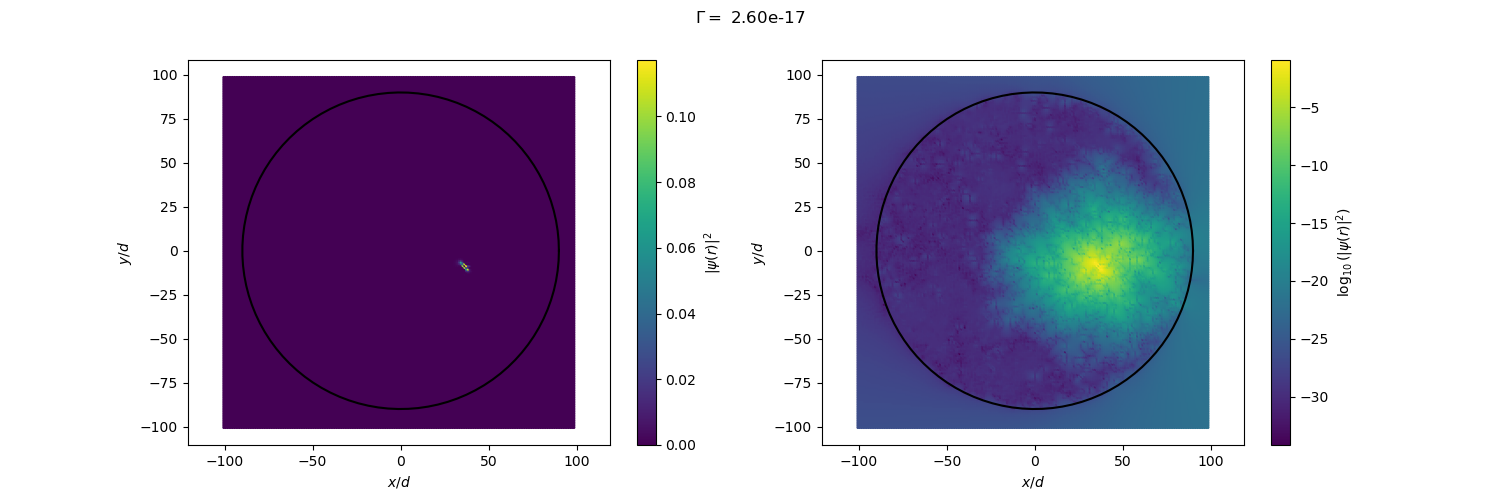
\includegraphics[width=1\linewidth]{img/loc_both.png}
    \caption{\textit{Left}: Wavefunction of a localized state with energy $E=0.005E_0$ and scattering length $a_{eff}=d$ in a lattice of radius $R=80d$ . \textit{Right} Logarithm of the wavefunction. }
    \label{fig:localized_state}
\end{figure}

Also, we can see that the inverse of the lifetime, or the $\Gamma$ is really small. Remembering that the lifetime of a state is $\tau=\frac{1}{\Gamma}$, we can see that the lifetime of the state is really long. This is a typical behaviour of a localized state, as the state is confined in a region of space in which the classical particles are not. We will say that a state is localized if the lifetime of the state is longer than $10^6$ times the characteristic time of the system, that is, if $\Gamma < 10^{-6}E_0/\hbar$.

The following found state, \cref{fig:border_state}, is a state with energy $E=0.005E_0$ and scattering length $a_{eff}=d$. This state is not localized, but for another reason: because the state is in the border of the system, its lifetime (or the mean time to escape the system) is shorter than the threshold. This is intuitive to think, as if the state is in the border of the system, it will have a higher probability of escaping the system.


\begin{figure}[ht]
    \centering
    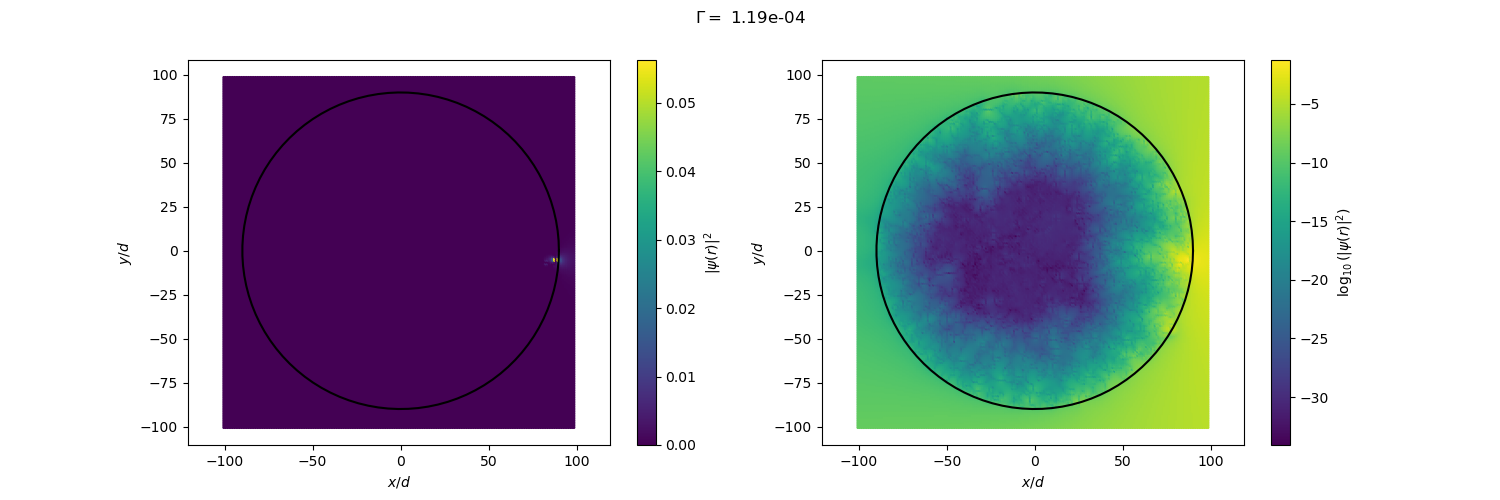
\includegraphics[width=1\linewidth]{img/Delocish.png}
    \caption{\textit{Left}: Wavefunction of a localized state with energy $E=0.005E_0$ and scattering length $a_{eff}=d$ in a lattice of radius $R=80d$ . \textit{Right} Logarithm of the wavefunction. }
    \label{fig:border_state}
\end{figure}

A complete delocalization of the state is shown in \cref{fig:deloc_state}. This state has energy $E=0.005E_0$ and scattering length $a_{eff}=d$. The state is spreaded through the whole system, and it is not localized.

\begin{figure}[ht]
    \centering
    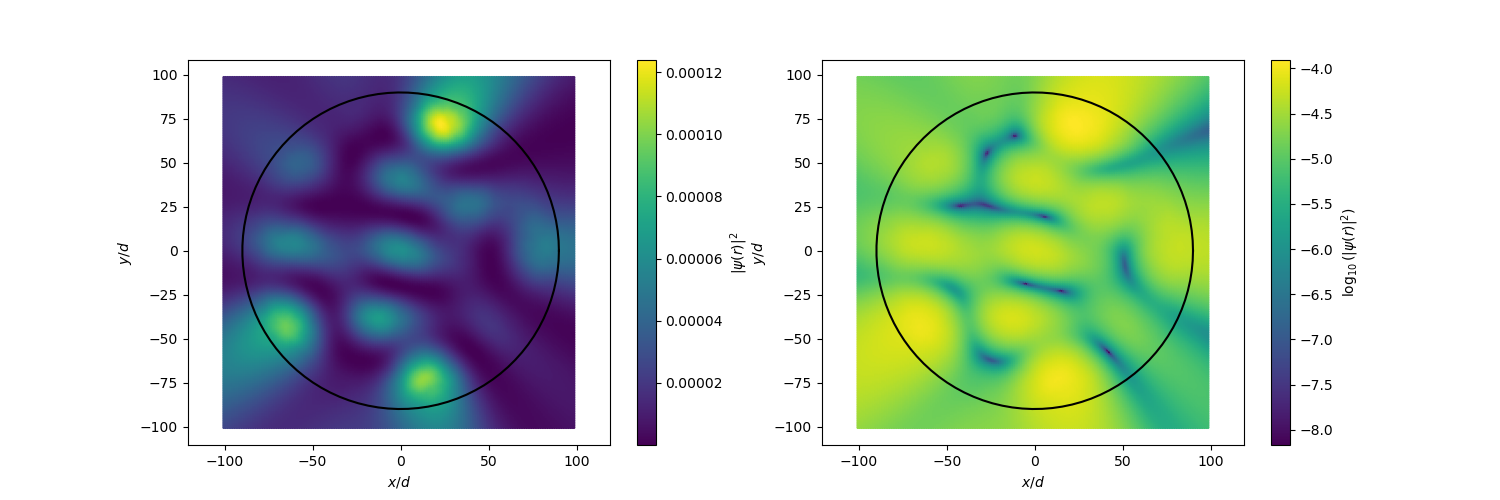
\includegraphics[width=1\linewidth]{img/other_deloc.png}
    \caption{\textit{Left}: Wavefunction of a surface state with energy $E=0.005E_0$ and scattering length $a_{eff}=d$ in a lattice of radius $R=80d$ . \textit{Right} Logarithm of the wavefunction. }
    \label{fig:deloc_state}
\end{figure}

As we see in the histogram \cref{fig:loc_states}, and can be observed also in \cite{antezzaQuantitativeStudyTwo2010}, as we increase the energy, the number of localized states decreases. An example of a delocalized state is shown in \cref{fig:high_energy}, with energy $E=0.5E_0$ and scattering length $a_{eff}=d$. The state is spreaded through the whole system.

\begin{figure}[ht]
    \centering
    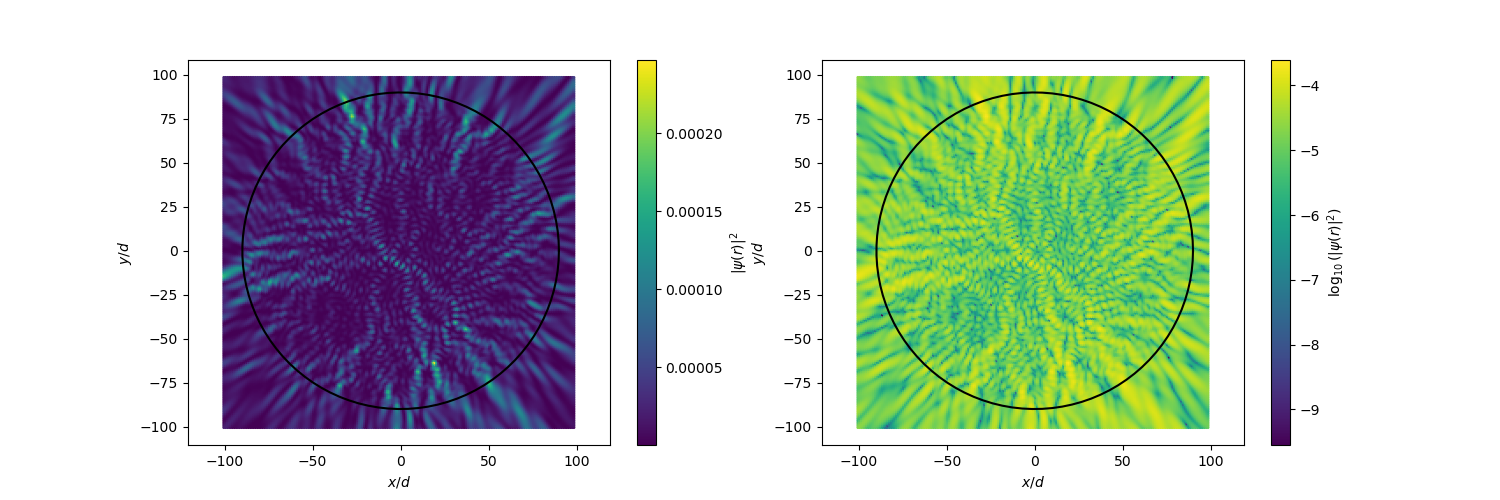
\includegraphics[width=1\linewidth]{img/high_energy0.5.png}
    \caption{\textit{Left}: Wavefunction of a delocalized state with energy $E=0.005E_0$ and scattering length $a_{eff}=d$ in a lattice of radius $R=80d$ . \textit{Right} Logarithm of the wavefunction. }
    \label{fig:high_energy}
\end{figure}

Finally, we have to remember that we were computing this inverse of the lifetime with a one step Newton method. This method is only effective for finding resonances with a small width. If at the energy selected, the initial eigenvalue is not small enough, the method will not converge. This is shown in \cref{fig:weird_state}, where we can see that the state is actually not localized, but the lifetime seems to be small. In the title of the plot we can see that the result is a negative inverse of a lifetime, which doesn't make sense. This is a clear example of the limitations of the method used.

\begin{figure}[ht]
    \centering
    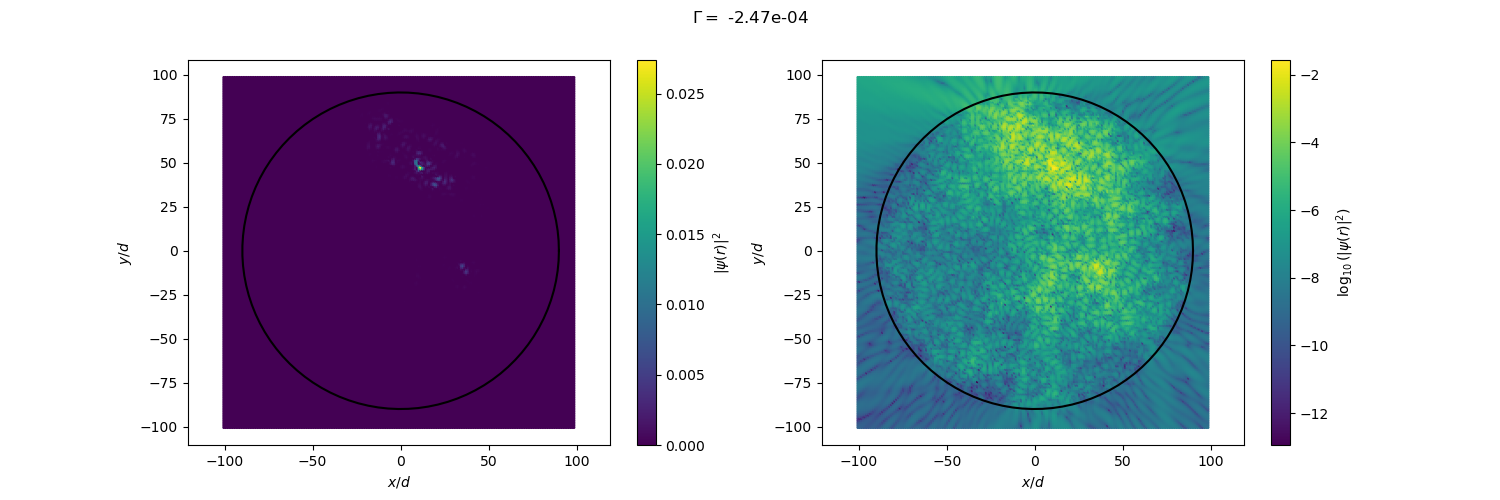
\includegraphics[width=1\linewidth]{img/Weird_semiloc.png}
    \caption{\textit{Left}: Wavefunction of a delocalized state with energy $E=0.5E_0$ and scattering length $a_{eff}=d$ in a lattice of radius $R=80d$ . \textit{Right} Logarithm of the wavefunction. }
    \label{fig:weird_state}
\end{figure}

% \begin{figure}
%     \centering
%     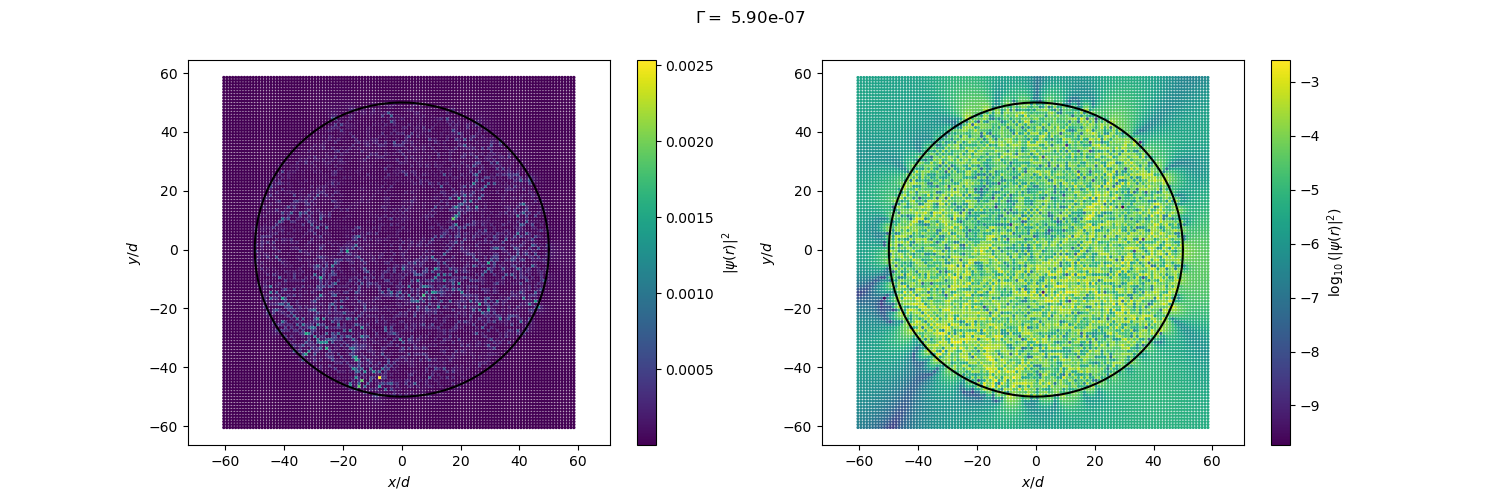
\includegraphics[width=1.2\linewidth]{img/0.9_occupation_lattice.png}
%     \caption{Number of states $N_i$ found for each bin $i$}
%     \label{fig:localized state}
% \end{figure}